\documentclass[journal,10pt,draftclsnofoot,onecolumn]{IEEEtran}

\usepackage{url}
\usepackage[tight,footnotesize]{subfigure}
\usepackage{amsthm}

% *** MISC UTILITY PACKAGES ***
%\usepackage{ifpdf}
% Heiko Oberdiek's ifpdf.sty is very useful if you need conditional
% compilation based on whether the output is pdf or dvi.
% usage:
% \ifpdf
%   % pdf code
% \else
%   % dvi code
% \fi
% The latest version of ifpdf.sty can be obtained from:
% http://www.ctan.org/tex-archive/macros/latex/contrib/oberdiek/
% Also, note that IEEEtran.cls V1.7 and later provides a builtin
% \ifCLASSINFOpdf conditional that works the same way.
% When switching from latex to pdflatex and vice-versa, the compiler may
% have to be run twice to clear warning/error messages.

% *** CITATION PACKAGES ***
%
%\usepackage{cite}
% cite.sty was written by Donald Arseneau
% V1.6 and later of IEEEtran pre-defines the format of the cite.sty package
% \cite{} output to follow that of IEEE. Loading the cite package will
% result in citation numbers being automatically sorted and properly
% "compressed/ranged". e.g., [1], [9], [2], [7], [5], [6] without using
% cite.sty will become [1], [2], [5]--[7], [9] using cite.sty. cite.sty's
% \cite will automatically add leading space, if needed. Use cite.sty's
% noadjust option (cite.sty V3.8 and later) if you want to turn this off
% such as if a citation ever needs to be enclosed in parenthesis.
% cite.sty is already installed on most LaTeX systems. Be sure and use
% version 5.0 (2009-03-20) and later if using hyperref.sty.
% The latest version can be obtained at:
% http://www.ctan.org/tex-archive/macros/latex/contrib/cite/
% The documentation is contained in the cite.sty file itself.

% *** GRAPHICS RELATED PACKAGES ***
%
\ifCLASSINFOpdf
  \usepackage[pdftex]{graphicx}
  % declare the path(s) where your graphic files are
  % \graphicspath{{../pdf/}{../jpeg/}}
  % and their extensions so you won't have to specify these with
  % every instance of \includegraphics
  \DeclareGraphicsExtensions{.pdf,.jpeg,.png}
\else
  % or other class option (dvipsone, dvipdf, if not using dvips). graphicx
  % will default to the driver specified in the system graphics.cfg if no
  % driver is specified.
  % \usepackage[dvips]{graphicx}
  % declare the path(s) where your graphic files are
  % \graphicspath{{../eps/}}
  % and their extensions so you won't have to specify these with
  % every instance of \includegraphics
  % \DeclareGraphicsExtensions{.eps}
\fi


% correct bad hyphenation here
\hyphenation{op-tical net-works semi-conduc-tor}

\newtheorem{mydef}{Definition}


\begin{document}

\title{Tracking the Diffusion of Named Entities}


\author{TBD}% <-this % stops a space

% The paper headers
\markboth{Computational Intelligence Magazine}
{Shell \MakeLowercase{\textit{et al.}}: Tracking the Diffusion of Named Entities}

% make the title area
\maketitle

% As a general rule, do not put math, special symbols or citations
% in the abstract or keywords.
\begin{abstract}
To do
\end{abstract}

% Note that keywords are not normally used for peerreview papers.
\begin{IEEEkeywords}
To do
\end{IEEEkeywords}

\IEEEpeerreviewmaketitle



\section{Introduction}

The aim of this paper is to understand how named entities \emph{emerge} and \emph{spread} through social media based discourse.
We are interested in exploring the following research questions:
\begin{enumerate}
	\item \textbf{RQ1:} How can we accurately detect named entities in social media based discourse, given its myriad formats, often informal vernacular, and inherent noise (e.g. misspellings, abbreviations, etc.)?
	\item \textbf{RQ2:} Under what conditions do entity mentions diffuse through discourse? And when are people \emph{most likely} to be influenced into then discussing entities?
	\item \textbf{RQ3:} How can we predict the discussion of certain named entities and who will begin talking about them?	
\end{enumerate}


\section{Datasets}
For this research we will use the following datasets:

\begin{enumerate}
	\item Reddit data -- download and access all of the data from the full dump.\footnote{\url{https://archive.org/details/2015_reddit_comments_corpus}}
	\item CoNLL 2003 data -- a corpus of newswire texts, annotated for named entity chunks and types.
	This describes where entity mentions are in the text, including locations, organisations, and person mentions.
	\item Twitter data; unannotated -- we have a large corpus of English tweets that we can use here.
	\item Twitter data; annotated -- there are two datasets annotated with named entities. These are from Ritter's 2011 EMNLP paper, and the W-NUT 2015 shared task.
\end{enumerate}


\section{Research Stages}

\subsection{Stage 0: Data Preparation and NER}
-To do:\\
--Annotate corpora with detected entities using basic typing of: person, location, organisation\\
--Run NER software over dataset and validate accuracy of this (using basic measures)\\
--Run NER over entire dataset to extract entities

\subsection{Stage 1: Exploratory Analysis}
-To do:\\
--Plot relative frequency distribution as a function of time for named entities, and characterise the \emph{shape} of the entities\\
--Apply lifecycle model to profile users' NER citations over time and investigate how users' profiles are influenced by global, community, and prior behaviour dynamics

\subsection{Stage 2: Diffusion Analysis}
-To do:\\
--Model the spread of named entities through user profiles (could use multivariate diffusion models here)

\subsection{Stage 3: Forecasting}
-To do:\\
--Implement models to forecast if a user will mention an entity and who that will be (hard!)


%-----------------------------------------------------

\section{Related work}
In this work we investigate how entities diffuse over time through the online community platform Reddit.
Diffusion of information is a well studied topic, and is of particular interest today given the myriad ways in which Web users consume information and are thus influenced by what they read, and with whom they interact with, online.

\subsection{Named Entity Recognition}
\textbf{TODO: Leon - add in existing works in NER that are relevant here}

\subsection{Information Diffusion}
Bakshy et al. \cite{bakshy2012role} conducted a large-scale randomised control trial to examine the effects of information exposure on information diffusion, using the Facebook platform.
The authors were able to assign Facebook users \emph{randomly} with a $1/3$ probability to the \emph{feed} group, and the remainder to the \emph{no feed} group and then \emph{hide} information (i.e. status posts) posted within the latter's group.
Bokshy et al. found, unsurprisingly, that users who were \emph{exposed} to information (i.e. those in the feed group) from their friends are more likely to share it on.

The closest work to the study of entity diffusion can be found in studies of hashtag diffusion.
For instance, Romero et al. \cite{romero2011differences} studied the spread of the top-500 hashtags posted in a sample of $>3B$ tweets collected over a six-month period, finding that users were most likely to \emph{adopt} a hashtag (i.e. mention/cite it in their Tweet) after receiving $4$ exposures from their friends.
The authors found marked differences in the adoption of hashtags based on their topics, something which - as we will show below - is not present in entity diffusion.

Goyal et al. \cite{goyal2010learning} track the diffusion of \emph{actions} on Flickr, where actions are users joining a group.
A general threshold model is proposed that determines the probability of influence between two arbitrary users based on the relative frequency of action propagation observed before between the users divided by the absolute number of actions of the user responsible for the propagation.
We use this general threshold framework, but extend it into the entity-mention setting, hence: we track the \emph{mention} of an entity by a user over time and calculate the probability of influence that an \emph{adopter}'s neighbours have had upon him.
Furthermore, we also extend this framework to test for two additional constructs: (i) influence of interactions before adoption (i.e. did the degree to which an individual communicated with a previous entity adopter influence their own adoption?), and (ii) community homophily (i.e. does the similarity between users' interests - based upon similarity in subreddit posting - have an effect on adoption of an entity?).

Fang et al. \cite{fang2013predicting} presented a method to predict adoption probabilities in social networks by controlling for potential confounding, unobservable variables - proposing a modification of expectation-maximisation to induce a Naive bayes predictive model.
The authors found that social influence alone is sufficient to recover the diffusion process, and thus external factors - that are latent - must be countered for within any predictive model, in the context of predicting the adoption of social ties.
Although such a framework allows one to control for confounding in the diffusion process, the study of the spread of entities is yet to be studied: hence in this work we aim to provide the \emph{first} effort in this space and to discern between the effects of social influence, interactions, and community homophily.




twitter info propagation

reddit compared to other OSNs: "Lifespan and propagation of information in On-line Social Networks: A case study based on Reddit"  http://www.sciencedirect.com/science/article/pii/S1084804515001307

network structure of reddit: "Navigating the massive world of reddit: using backbone networks to map user interests in social media" https://peerj.com/articles/cs-4/

twitter nlp


\section{Data preparation and NER}

To conduct our study, we need to convert 140GB of compressed Reddit posts into a set of interlinked and time-ordered conversations and the entities mentioned in each of them.
This provides a number of sub-challenges: sampling of the Reddit data, creating a linked series of conversations, and picking out entity mentions in this text type.
Reddit data is largely unexplored in the NLP community, despite the large volume of it and the especially rich metadata.
This poses additional challenges: certainly, given the lack of work on Reddit text, there are no annotated datasets available yet, so supervised in-domain work is not directly possible yet.
Additionally, the datasets are large, which makes it important to choose a good subset of data on which to do prototyping and development, in order to keep research cycles short.
The result that we come to at the end of this stage is a rich dataset for tracking entity and concept diffusion within and across communities.

\begin{figure}
\centering
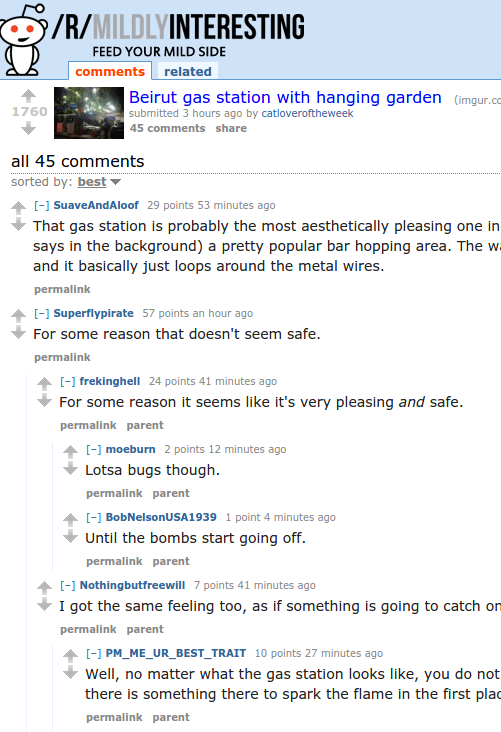
\includegraphics[width=0.4\columnwidth]{reddit-example.png}
\label{fig:reddit-example}
\caption{Example discussion around a Reddit post.}
\end{figure}

The Reddit dataset~\cite{reddit-data} is comprised of a sequence of comments, with one JSON record for each one.
These are ordered temporally.
Reddit itself is roughly similar to a forum, where top-level divisions are made by topic.
Within each topic, or {\em subreddit}, there are posts, which begin with either a short piece of text or a link to an external resource -- typically an image, video, or interesting article.
Users then may publish comments for each post, and reply to each others' comments.
This leads to a threaded discussion, centred on a particular topic, with a hierarchical comment structure (see Figure~\ref{fig:reddit-example}).


\subsection{Subreddit extraction}

- subreddit extraction

top lists

describe top lists site

pick 100

extract these over whole sample

figures for raw dataset (\# per year; total volume over time; volume-rank graph of subreddits; possible ref to appx)

\subsection{NER for Reddit}

-- where is NER first mentioned and defined?

We model micro-topics in conversation as entity mentions.
This allows tracking of topics at maximally fine granularity, looking at each user's interests at a low level, as opposed to monitoring broader topics such as ``consumer electronics", ``politics" and so on.
In fact, these broader topics are already explicitly annotated by means of the subreddit topics.

Entity mentions are extracted through named entity recognition.
Generally, this task aims to detect the boundaries of certain kinds of entities within a certain piece of text.
In this instance, we tokenise text, splitting it into sentences using the Punkt tokeniser~\cite{kiss2006unsupervised}, and subsequently word-sized chunks, using the {\tt twokenize} tool with some adaptations~\cite{o2010tweetmotif}.
This tool performs Penn Treebank-style tokenisation, a common standard, with some specific adaptations to enable it to handle the noise present in user-generated text.
After this, we take a structured prediction approach to deciding which tokens in each sentence are part of an entity, and possibly the type of the entity.
Finally, we concatenate entity tokens, and use these to build a list of entity mentions in any given input text.
For example, given the input comment from the source JSON:

\begin{quote}
\emph{``body": ``There are still some really good fighters on this card. Conor McGregor is on the card and so is Gunnar Nelson."}
\end{quote}

The following output entities should be collected:

\begin{quote}
\emph{``entity\_texts": [``Conor McGregor", ``Gunnar Nelson"]}
\end{quote}

Typically, many NER systems take a supervised approach; that is, they use data labelled by humans as training data, from which features are extracted to form training instances for a machine learning algorithm.
However, NLP systems can be hard to transfer between text types; for example, NER systems for newswire might reach about 89\% F1 on news articles, but only around 40\% on tweets (a form of user-generated content), as found in~\cite{derczynski2015analysis}.
One approach to overcoming this performance drop when changing text type is to train over a blend of text types.
For example, Ritter~\cite{ritter2011named} used both IRC\footnote{Internet Relay Chat -- informal internet conversation text} and newswire data when developing a part-of-speech tagger for tweets, as well as an unsupervised language model from the target text type.
This led to strong performance improvements.
We follow a similar approach, using a blend of NE-annotated corpora from both newswire and tweets.
The newswire data is drawn from the CoNLL-2003 evaluation task set~\cite{tjong2003introduction}; the twitter data is from Ritter's early experiments and also the W-NUT 2015 shared task~\cite{ritter2011named,baldwin2015shared}.

We start using structured predicting in the form of a CRF to label whole sentences at a time.
For features, we use a fairly classical set, and add some unsupervised word representations to this.
Our base features are:

\begin{itemize}
\item 
\end{itemize}

In addition, we induce Brown clusters~\cite{brown1992class} and use these as word representations~\cite{turian2009preliminary}.
Brown clustering is a form of hierarchical agglomerative hard clustering, using average mutual information as its objective function.
It takes as input a corpus, in the form of a sequence of words, and in its generalised form~\cite{derczynski2016generalised}, a single hyperparameter: the size of its active set $a$.
The result is a sequence of binary merges, describing the set membership of each word type in the corpus as the merges progress.
For each single word type, therefore, the path to a destination cluster can be described as a bitstring, which details the sequence of binary merges taken.
The zero-length bitstring describes the situation at the top of the hierarchy, where there is one class.

These bitstrings are typically converted to features by shearing.
This involves only examining the first $n$ bits of a bitstring.
However, shearing does not maximise the information preserved in the representation -- sub-clusterings at many levels are lost.
We therefore experiment with a new method of feature extraction form Brown clusters, which we call {\em provenance-based} feature extraction.
We take the cluster identifier at every level, tracing the provenance of a terminal word cluster all the way to the root cluster (which contains all word types).
This preserves the entire set membership of any given term, throughout the induced hierarchical clustering.
As an example, if the term \emph{fishing} has bitstring {\tt 1100101}, the following text features are generated: {\tt 1}, {\tt 11}, {\tt 110}, {\tt 1100}, {\tt 11001}, {\tt 110010}, {\tt 1100101}.
For contrast, if the typical bit depths of 4, 6, 10 and 20~\cite{ratinov2009design} were chosen, only the following features would be generated: {\tt 1100}, {\tt 110010}, {\tt 1100101}.
As a result of taking all directly-relevant features in the merge list, the lossy nature of shearing-based feature extraction from Brown clusters is avoided.

Feature extraction, training, classification and JSON annotation are all performed using an entity recognition toolkit (https://github.com/leondz/entity\_recognition~\cite{derczynski2015usfd}), with custom extractors.


\subsection{Tuning entity recognition}

Entity recognition needs to be tuned to fit Reddit data well.
There are a number of parameters in our training data balance, feature extraction, and objective function that all reflect the nature of the data and the task at hand.
We present our method for estimating of these factors, and intrinsic NER evaluation.

In terms of evaluation, we prefer recall over precision.
Over the large dataset, spurious entities are likely to be those that are not seen very often or have an unusual pattern.
This suggests that there will be great variation in their surface forms, leaving them in the long tail of discovered entities.
As the majority of our work looks at the more frequent patterns, these are less likely to have an impact.
Conversely, recall reveals how well the extraction is performing, and it important to track a range of entities.
In addition, recall has always been more challenging to achieve in social media texts than recall~\cite{ritter2011named,derczynski2015analysis}.

To capture this balance, we take F-scores with $\beta=2$.
Given precision $P$ and recall $R$, typically an F-score is drawn from $F_\beta$ with $\beta=1$.

\begin{equation}
F_\beta = (1+\beta^2)\frac{PR}{(\beta^2 P) + R} 
\end{equation}

When $\beta=1$, precision and recall are balanced in a harmonic mean, e.g. F1-score.
That is, false positives and false negatives impact results equally.
To score away from false positives, i.e. wrong cues, we set $\beta=2$.

Our approach here is to tune an entity recogniser with reference to a dataset that matches the target text type.
We draw this development set from Reddit posts, using comments encountered during our work that appear to have missing or spurious annotations.
These are then isolated, tokenised, and manually annotated.
Our annotation format follows~\cite{ritter2011named} in using the Freebase top-level entity type inventory, but only uses the chunking information, as nothing further than this is needed: only the surface forms of entities.
In total, we identified and annotated 3\,708 tokens of Reddit data, including 149 entity chunks.
This comprised our development set, which was used to tune a variety of parameters in our approach.

Firstly, we tuned our word representations.
Specifically, we needed to estimate the number of Brown clusters $C$ to use in feature extraction.
We also then used this to determine what blend of social, Reddit or news data gave best results in unsupervised feature generation and extraction.
To tune the value for $C$, we examined a similar scenario with similar dataset sizes, and estimated an optimum.
We noted that in prior work~\cite{derczynski2015tune}, entity recognition performance with decomposed class prefixes -- similar to the provenance-based features we propose here -- peak at around $C=2500$ for corpora of 16k tokens, $C=5000$ for corpora of 32k tokens, and at higher values for larger datasets.
As General Brown clustering is dependent on the number of types and the size of the active set $a$, and results are unreliable with $a>C$, we set $C = a = 4000$.
We then experiment with combinations of newswire, Twitter and Reddit data.
Brown clusters are extracted using the generalised-brown package~\cite{sean_chester_2015_33758}.
Results are given in Table~\ref{tab:brown-tuning}.

-- results of brown cluster tuning


In addition, we draw supervised data for multiple datasets in order to approximate the Reddit text type.
We take data from Reddit, taking the union of corpora used in previous work that follow the Freebase ten-class entity scheme~\cite{ritter2011named,baldwin2015shared}.
This scheme gives broader coverage than e.g. the three-class ACE named entity scheme.
For newswire, we use the Reuters RCV1 corpus annotations that were part of the CoNLL-2003 shared task~\cite{tjong2003introduction}.
Classes are removed before training, making this just a chunking task.
We compare against Stanford NER~\cite{finkel2005incorporating} as a baseline.
Results for different balances of training data are given in Table~\ref{tab:supervision-balance}


-- analysis of cross-genre ne chunking performance


Note that while some figures seem low when compared to typical newswire level performance, the toolkit used is high-ranking, state-of-the-art research software, coming third in the 2015 W-NUT challenge for entity chunking over tweets.
The task is simply difficult; Twitter NER recall has always been low.
In addition, it is a generally consistent finding that generalising NER systems beyond newswire is not yet well understood; systems that perform very well on this text type (e.g. F1 of 0.89 from Stanford NER~\cite{derczynski2015analysis}%~\cite{derczynski2013microblog}
) can often score very poorly on social media content (F1 of 0.41).
This may be due to overfitting of tools to newswire over time, due to community challenges, dataset in just one type, extra custom rules adapting to formal news text, or other things -- but this is beyond the scope of this paper.
We do note that our approach uses largely unsupervised feature extraction and performs better than on other social media corpora, also beating the Stanford NER system, in this first attempt at named entity chunking for Reddit.


\clearpage
\section{Entity Diffusion}
In this section we now move on to examining how the recognised entities emerge and \emph{diffuse} through the analysed subreddits.
As per prior work, one of the first things that we can inspect is the \emph{shape} of entity mention cascades: that is, the patterns of diffusion that such entities exhibit when cited in conversation chains. 
We begin by explaining how such patterns are derived, before then moving on to showing that patterns emerge.

\subsection{Entity Mention Cascades}
Prior work by Leskovec et al. \cite{leskovec2007patterns} examined the shapes of hyperlink cascades through the blogosphere; in doing so, investigating that patterns appear in terms of the diffusion of links.
We follow a similar process here, however we instead inspect the emergence of entities in conversation chains in reddit.
We first make the following explicit.

\begin{mydef}
(Entity Cascade) A cascade of ${<p_i, pj>} \in C_e$ of an entity $e \in E$ occurs when two or more posts citing the entity are chained together in a reply graph. 
Hence: $C_e = \{<p_i, p_j> : p_i \rightarrow p_j \in R, cites(p_1) = cites(p_j) = e\}$.
\end{mydef}

Our goal is to derive all entity cascades for each entity in our analysis, and then examine how the shapes and sizes of these cascades differ.
To gather each entity's cascades, we retrieved all subreddit posts that contained a given entity.
For each post ($p \in P_e$), we then recovered the reply-chain that that entity appeared within - this was performed by going \emph{up} the reply chain from $p$ to its parent post (i.e. the post that $p$ was replying to) and \emph{down} the reply chain by getting the posts that replied to $p$.
When iterating through the posts, if we came across a post that replied to another post in an existing chain then that post was added to the chain.
We only maintained posts within the chain that cited the entity in question: this produced entity cascades where each consecutive post in the chain mentions the entity - we refer to this as \emph{strict cascade derivation}, as we do not consider posts higher-up or lower-down the reply chain that cite the entity yet are connected by a non-entity citing post. \footnote{The Python code for deriving these chains is available at the following URL: \url{https://github.com/mattroweshow/NER-Diff-Paper}}

This process produces, in essence, a collection of cascade graphs for each entity, each of which may have isomorphic shapes yet contain different node labels (i.e. different post ids).
We reduced each entity's cascade graph collection down to a frequency distribution of the \emph{canonical form} of each graph using Cordella at al.'s \cite{cordella2001improved} graph isomorphism approach.
A further reduction was run to compile a frequency distribution of the cascade shapes across all entities.
Fig. \ref{fig:entity_cascades} show both the top-20 entity cascade shapes on the left (Fig. \ref{fig:cascade_shapes}) and the ranking of the patterns' frequencies on a log-log scale (Fig. \ref{fig:rank_dist}).
Upon inspection, one thing becomes immediately apparent: entity cascades are shallow and short at the top-3 ranks, however after this position we start to see chains of discussions as being popular which are deeper and narrow.
This result contrasts somewhat to prior work \cite{leskovec2007patterns} where cascades of hyperlinks between blogs were shallower in depth yet wider - in terms of the breadth of diffusion at the first level from the seed. 
The ranking of the patterns follows a general power-law distribution where a small section of patterns (i.e. the top-20) are seen most often - this is somewhat expected as it would be very rare for an entity to be cited in a long thread with many branching reply-chains.

\begin{figure}[ht!]
  \begin{center}
  \subfigure[Top-20 Cascade Shapes]{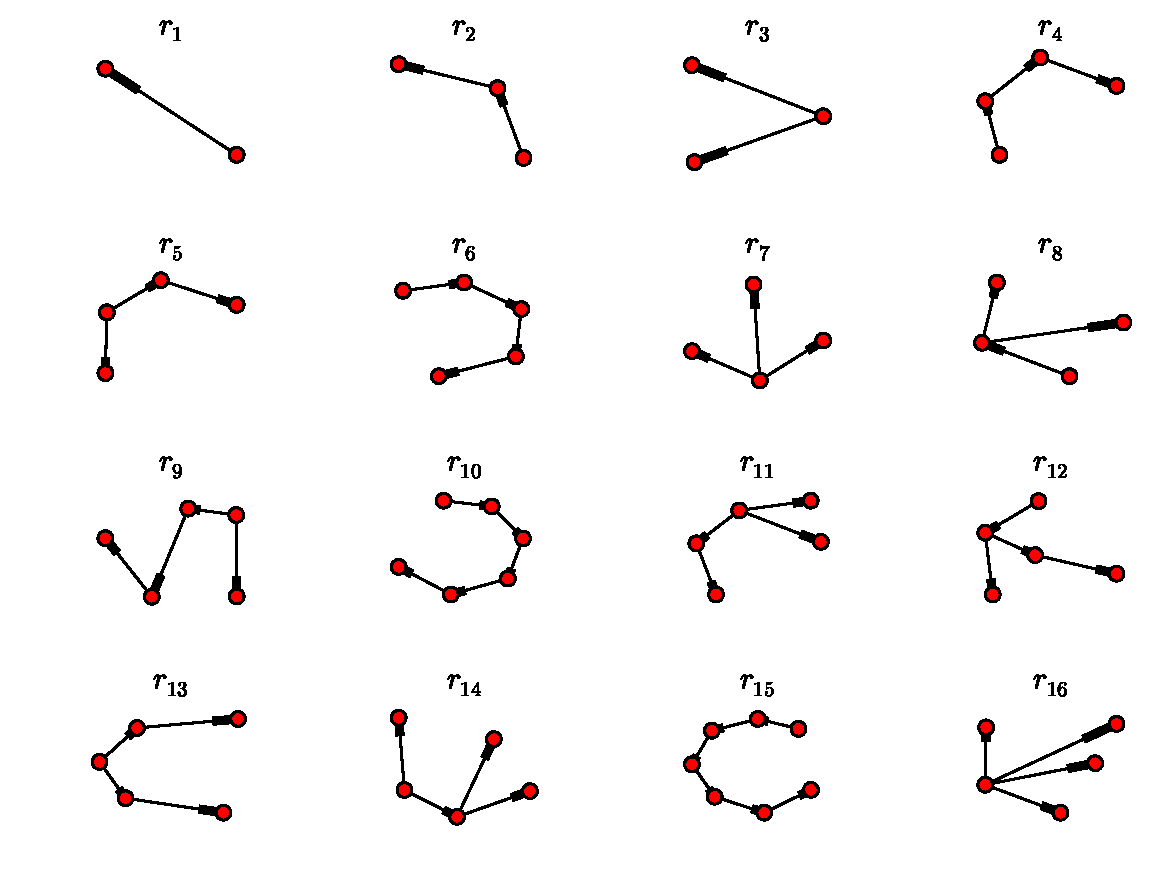
\includegraphics[width=0.49\columnwidth]{plots/cascade_shapes.pdf}\label{fig:cascade_shapes}}   
  \subfigure[Cascade Shape Rank Distribution]{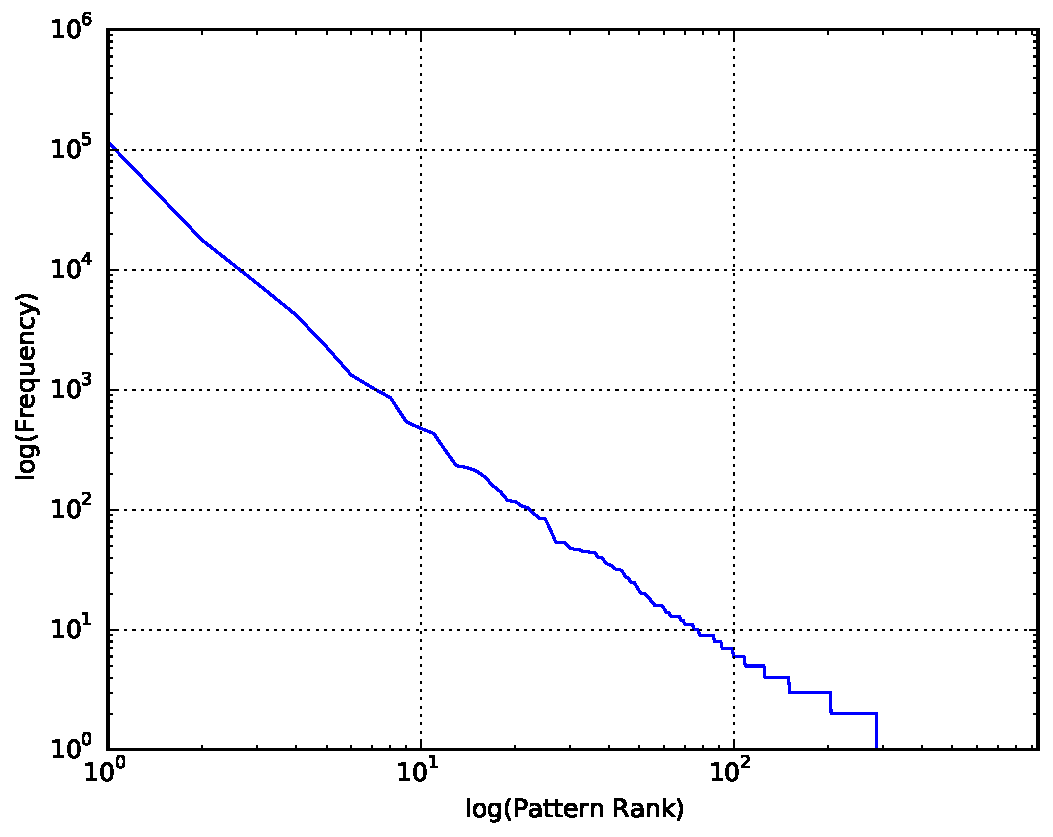
\includegraphics[width=0.49\columnwidth]{plots/cascade_rank_dist.pdf}\label{fig:rank_dist}}
  \end{center}    
  \caption{The top-20 cascade shapes are generally deep and narrow with little branching (Fig. \ref{fig:cascade_shapes}, while the cascade shape rank follows a power-law distribution (Fig. \ref{fig:rank_dist}.}
  \label{fig:entity_cascades}
\end{figure}

\subsection{Entity Adoption Post-$({k-1})^{th}$ Exposure}
Inspection of the shape of entity cascades through Reddit discussion threads reveals some interesting traits, suggesting that an entity is likely to be a adopted if it has been discussed \emph{a priori} within the same discussion thread.
One natural question that emerges from this is the extent to which exposures to entities play a role in actually adopting (i.e. citing) the entity in question.
To investigate the relationship between exposures and adoptions, we sampled the top-500 entities from our whole annotated dataset and calculated the probability of a user adopting an entity after being \emph{exposed} to the entity $k$ times.

\begin{mydef}
\label{def:exposure}
(Exposure) A user $u$ is exposed to an entity $e$ at time $t$ if a given post $p \in P^{\Gamma(u,t}$ authored by a neighbour of $v \in \Gamma(u)$ contains the entity $e$, where neighbours of $u$ are those users that he interacted within prior to $t$.
\end{mydef}

Based on this definition we iterated through all posts chronologically that cited a given entity, and if the post was the first time that a user cited the entity (i.e. he/she was not \emph{activated}) then we counted how many \emph{exposures} the user had received prior to the time of the post - logging this as $k$.
Fig. \ref{fig:global_exposure_dist} present the \emph{overall} plot of the probability (i.e. relative frequency) of users adopting an entity after $k$ exposures to the entity.
Immediately, one can note that the mode of this distribution is at $0$ and that the mean if $k=23$: this implies that users are most likely to actually cite an entity without having been exposed to it, in fact $P(adoption) \rightarrow 0, k \rightarrow \infty$.
We are somewhat guarded in \emph{generalising} from this result, as our experimental setup here - given the scale of the data we are playing with and the tractability of annotating the entirety of Reddit - does result in only a fraction of Reddit being annotated with entities.
Hence, it is possible that entities emerge from other subreddits, yet we are unable to capture this at present - our future work makes suggestions as to how this effect can be validated.
Furthermore, this finding contrasts somewhat to existing patterns of \emph{hashtag} adoption \cite{romero2011differences}: in hashtag adoption, there is a clear mode at around $k=4$ exposures, after which the probability of adoption curtails.
This difference is likely due to two factors: firstly, the differences of the platforms - as Twitter acts as a public broadcast spectrum where information is presented in feeds and is then passed on, while Reddit is more interaction and discussion-driven, and; secondly, the manner in which users are \emph{exposed} to information - on Twitter this via subscriptions to other users and observing trends in the trending topics area, while Reddit requires users to read through threaded discussions and \emph{notice} entities within.

The second plot below (Fig. \ref{fig:entity_exposure_dists}) shows a sample of 9 entities' adoption-exposure distributions, all of which have similar shapes (with a mode at $0$) and a heavy-tail.
Variance exists, however, in the means that these distributions have, for instance the entity \emph{PS1}\footnote{Denoting the original Playstation video-games console.} has a much lower mean than the entity \emph{Hungary} suggesting that users require less stimulation to discuss the former than the latter.
The nature of how and why the distributions differ is something that requires further investigation - for instance, clustering the entities per-topic and then examining the \emph{pooled} exposure-adoption graphs would allow one to understand topic-level patterns of spread (in a similar vein to \cite{romero2011differences}).


\begin{figure}[ht!]
  \begin{center}
  \subfigure[Exposure-Adoption Global Distribution]{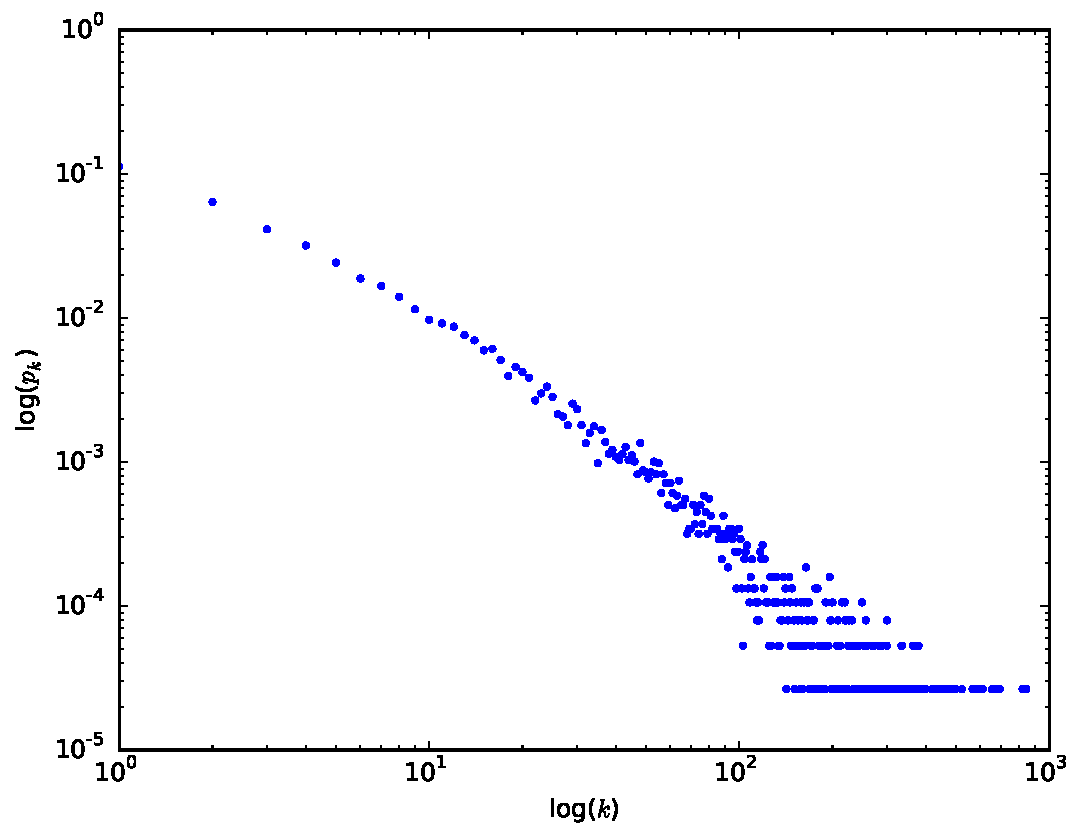
\includegraphics[width=0.49\columnwidth]{plots/exposure_count_dist_full_log.pdf}\label{fig:global_exposure_dist}}   
  \subfigure[Sampled Entity Exposure-Adoption Distributions]{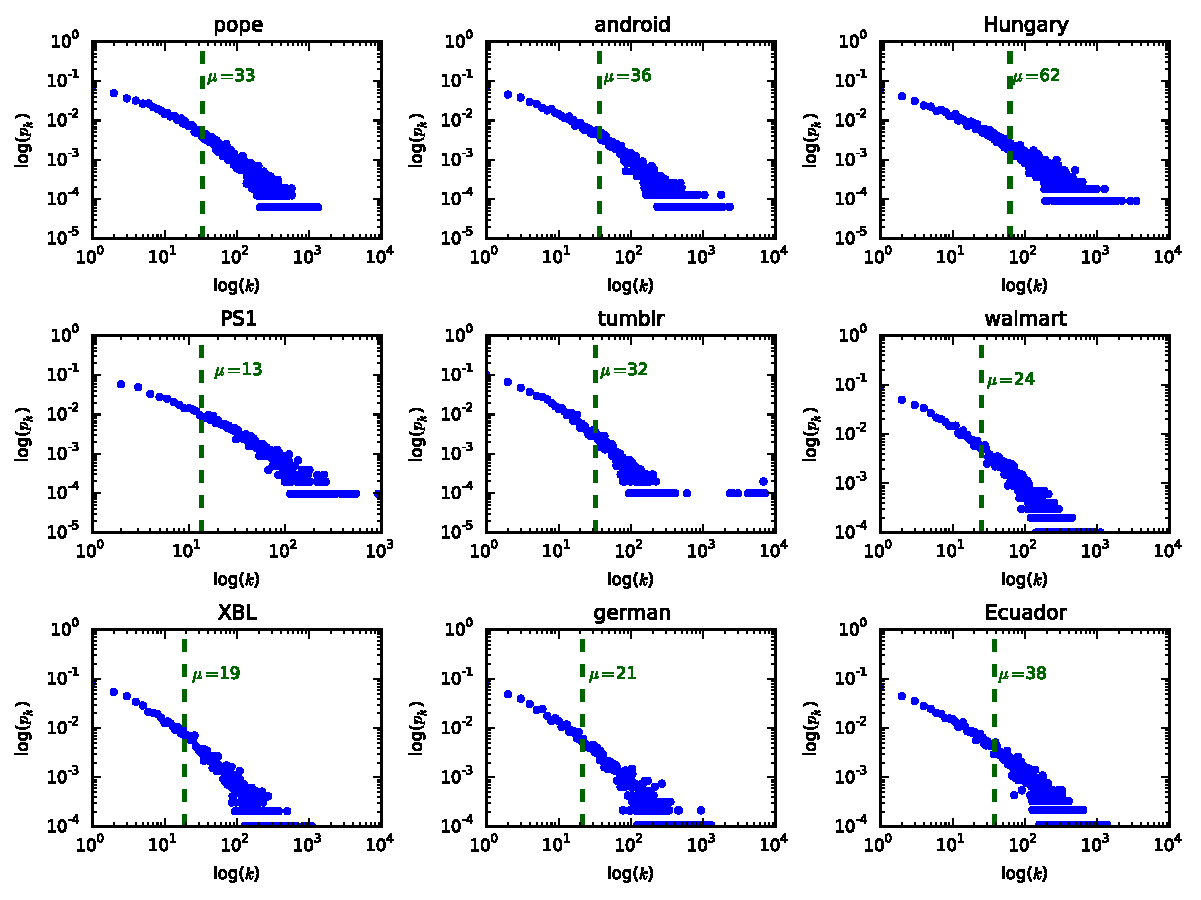
\includegraphics[width=0.49\columnwidth]{plots/per_entity_exposure_count_dist_full_log.pdf}\label{fig:entity_exposure_dists}}
  \end{center}    
  \caption{The probability of a user adopting an entity as a function of $k$ prior exposures to the entity has a heavy-tailed distribution (Fig. \ref{fig:global_exposure_dist}) that is consistent across all entities, including a sample of 9 random entities (Fig. \ref{fig:entity_exposure_dists}).}
  \label{fig:exposure_dists}
\end{figure}


\subsection{Global Threshold Diffusion Model}
We now move on to forecasting the diffusion of entities across Reddit.
For this, we use a modified implementation of Goyal et al.'s general threshold model \cite{goyal2010learning} to parallelise the computation of the model.
The core principle of the model is that one can calculate the probability of a user ($u$) adopting an entity ($e$) based on how his neighbours ($v \in \Gamma(u)$) have influenced him previously.
Hence, the probability of $u$ adopting an entity is calculated as follows:

\begin{equation}
\label{eq:joint_prob}
p_u\big(\Gamma(u)\big) = 1 - \displaystyle\prod_{v \in \Gamma(u)}\big(1 - p_{v,u}\big)
\end{equation}

In Goyal et al.'s prior framework, the probability of influence ($p_{v,u}$) of $v$ on $u$ is based upon the maximum likelihood estimate of a single Bernoulli trial.
An entity propagation occurs between $v$ to $u$ when when the latter cites $e$ after being exposed to it by the former (as per Definition \ref{def:exposure}), hence a count of how many entities propagate between $v$ and $u$ can be recorded in $E_{v2u}$.
From this, the influence probability between $v$ and $u$ based on such \emph{propagation} can be calculated as follows, where $E_v$ is how many times $v$ has cited an entity:

\begin{equation}
\label{eq:action_prob}
p^{E}_{v,u} = \frac{E_{v2u}}{E_v}
\end{equation}

The authors explain how there are two variants of this calculation: (i) a static Bernoulli random trial where Equation \ref{eq:action_prob} is calculated from the training set (ignoring time), and: (ii) a discrete time Bernoulli random trial where counts are only placed within $E_{v2u}$ and $E_v$ if they the citation of an entity is within a discrete time interval, that is: if the time that $u$ adopts an entity $e$ is given by time $t_u$ then $E_{v2u}$ and $E_v$ are composed from the entity posts of $v$ which each have time $t_v \in [t_u - \tau_{v,u}, t_u)$, where $\tau_{v,u}$ is derived as follows (only considering $v, u \in U$ (set of all users) if $u$ has contacted $v$ prior to $t_u$:

\begin{equation}
\tau_{v,u} = \frac{\displaystyle\sum_{e \in E} (t_u(e) - t_v(e)}{E_{v2u}}
\end{equation}

Fig. \ref{fig:taus_hist} shows the binned distribution of the $\tau_{v,u}$ values (reduced from milliseconds to hours to ease legibility): one can note how the distribution has a right skew with the mode of the distribution (roughly) being at one hour - that is, the majority of \emph{influence} from one person to another occurs within one hour, this then gradually curtails off with fewer people having larger \emph{influence windows}.
The log-log plot of the relative frequency distribution (Fig. \ref{fig:taus_loglog}) shows the \emph{heavy-tail} property of the distribution, and that the mean window width is $10,780$ hours ($\approx 449$ days $\approx 1.2$ years), thus suggesting a degree of \emph{stickiness} in the Reddit communities where people remain for long periods.


\begin{figure}[ht!]
  \begin{center}
  \subfigure[Binned Frequency Distribution of $\tau_{v,u}$ values]{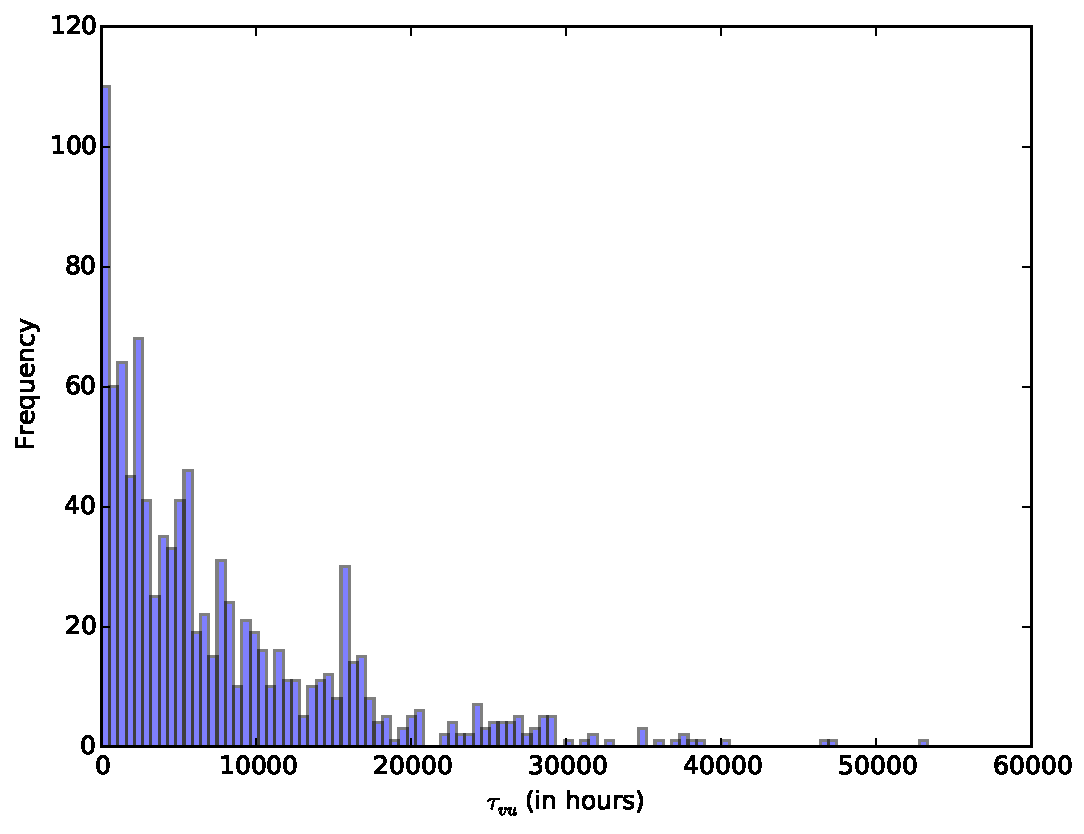
\includegraphics[width=0.49\columnwidth]{plots/taus_dist.pdf}\label{fig:taus_hist}}   
  \subfigure[Log-log Plot of the Binned $\tau_{v,u}$ distribution]{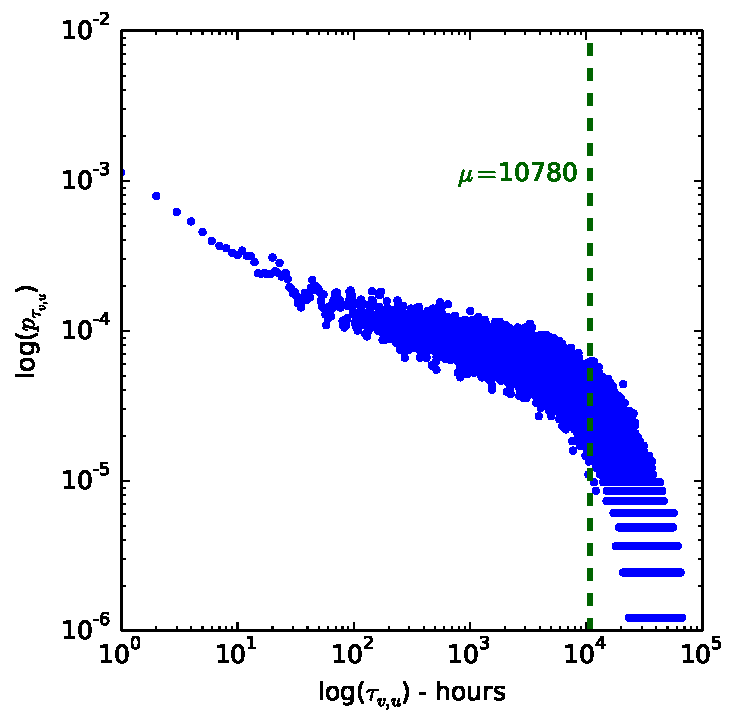
\includegraphics[width=0.49\columnwidth]{plots/taus_dist_full_log.pdf}\label{fig:taus_loglog}}
  \end{center}    
  \caption{The influence window ($\tau_{v,u}$) between two arbitrary users characterises the average time for an entity to propagate from $v$ to $u$. In hours, this value has a \emph{right-skew} (Fig. \ref{fig:taus_hist}), while the log-log plot (Fig. \ref{fig:taus_loglog}) of the relative frequency distribution demonstrates the heavy-tail nature of the distribution with a mean of $10,780$ hours ($\approx 449$ days $\approx 1.2$ years).}
  \label{fig:taus}
\end{figure}

\subsubsection{Additional Influence Dynamics}
The neat formulation of the general threshold model, and the monotonic-submodular nature of the probability of adoption function ($p_u(\Gamma(u)$), means that we can vary the mechanism by which we derive the \emph{influence probability} ($p_{v,u}$) between two user $v$ and $u$ to test for different influence effects.
Our contribution here is to test for the influence of \emph{prior interactions} and \emph{community homophily} using the general threshold model.
To compute the influence probability based on interactions, we derive $p^I_{v,u}$ as follows:

\begin{equation}
p^{I}_{v,u} = \frac{\vert \{ p_u : p_v \in P_v, p_u \in P_u, p_u \rightarrow p_v \} \vert}{\vert \{ p_u : p_u \in P_u, p_u \rightarrow . \} \vert}
\end{equation}

While the influence probability based upon community homophily ($p_{v,u}^C$ is derived as follows:

\begin{equation}
p^C_{v,u} = \frac{\vert C_u \cap C_v \vert}{\vert C_u \cup C_v \vert}
\end{equation}

We calculate the same two variants as the entity-propagation influence probability as above (static Bernoulli, and discrete-time Bernoulli) for these influence probabilities by only considering interactions between $u$ and $v$ that fall within $[t_u - \tau_{v,u}, t_u)$ (for interactions-based) and posts within subreddits by $u$ and $v$ that were made within $[t_u - \tau_{v,u}, t_u)$ (for community-homophily).

In order to eliminate bias in our below experiments - when we attempt to forecast entity adoption for users - we divided the top-500 entities into an 80\%:20\% split for training and testing respectively.
Then, for the above influence probabilities (entity-propagations, interactions-based, community-homophily) we used different strategies for their calculation.
For the entity-propagation influence probability ($p^E_u(S)$) we used the training segment to calculate the values of $E_{v2u}$ and $E_v$, and also $\tau_{v,u}$ - for all pairs of interacting users within the training segment - this follows the experimental setup of \cite{goyal2010learning}.
One thing that is somewhat limited about this approach, is that we are observing future effects when calculating $E_{v2u}$ and $E_v$ that we take forward into our experiments, as we observe how influence has occurred between users prior to an adoption happening.
To some extent, this is somewhat unavoidable in the context of the dataset splitting as $\tau_{v,u}$ must be calculated somehow - an alternative for future work here is to use a fixed time-split and use the first 80\% of entity-posts for training and the rest for testing - this does somewhat limited the generalisation capability however as new entities that appear in the latter portion would have limited information to learn their patterns of diffusion from.

\subsection{Experiments}
As mentioned above, one of our goals here is to \emph{forecast} the adoption of entities by users as their spread through Reddit.
To this end, we used an experimental setup that induces the joint probability function (Eq. \ref{eq:joint_prob}) for the users citing entities within the test set by tracking their probability of adopting a given entity as a function of their neighbours influence.
Our goal therefore is to examine which of the above influence probability functions are best suited to predicting adoptions.
We now explain our experimental setup before moving on to present the results of such models.

\subsubsection{Experimental Setup}
Using the 100 randomly sampled subreddits and running the above Named Entity Recogniser over these subreddits' posts, resulted in a total of XXX posts in our dataset (using only those from the 100 subreddits) written by 4,139,814 users - the entity recogniser also extracted 8,797,271 entities.
Of those users we had 2,745,311 user-to-user edges derived from XXX interactions.

\paragraph{Deriving Adoption Probabilities}
In order to test which model was best (from above) we took the entities within the test set, and ran the following process: we chronologically ordered each entities' posts and then iterated through the posts set one-by-one.
For each post's author ($v$) we then checked if he had been \emph{activated} before - i.e. had he cited the entity? - if not, then this would be first time he had cited $e$.
If this was the case then we retrieved the prior interactions that the user had had and calculated (for each prior neighbour - $u \in \Gamma(v, t_u)$) the probability of influence between $v$ and $u$ using the above influence probability variants (e.g. interactions-based with static Bernoulli setting).
We then updated the probability of adoption of $u$.
By iterating through the set of time-ordered posts we maintained adoption-outcome tuples of the form $<u, p_u, r_u>$ where $r_u \in \{0,1\}$ denoting whether the user ultimately adopted the entity $e$ or not.
Our evaluation of the models used these tuples to calculate the area under the Receiver Operator Characteristic curve, aiming to achieve a value of $1$ (for perfect prediction - with $0.5$ being the random model baseline.

\paragraph{Parallelising Processing}
As we are working with \emph{big data} here, we made two efforts to parallelise the processes above - induction of adoption probability over the test set entities.
First, all of the data used for the experiments (timestamped interactions between users, entity posts, post details, $E_{v2u}$ values, $\tau_{v2u}$ values) was uploaded into HBase\footnote{\url{https://hbase.apache.org/}} tables ensuring that we could \emph{quickly} access the data using time-specific queries (e.g. \emph{return all interactions where $u$ is the source before 12th January 2010}).
Second, we used Apache Spark\footnote{\url{http://spark.apache.org/}} to parallelise the per-entity diffusion processes.
This was performed by loading the names of the test entities into HDFS and then forcing Spark to partition the entity list into at least 30 partitions.
Each partition was then iterated over and the the above test process run: (i) retrieving time-ordered entity posts from HBase, (ii) iterating over the post set, (iii) retrieving per-user interactions prior to the time of a given post, (iv) calculating the pairwise influence probabilities.
The final calculated probability of adoption for each user ($u$) together with the label of whether they adopted the entity or not were recorded in a separate HBase table of results.

Unfortunately, due to the use of sample of 100 of the top-500 entities in our experiments, iteration over the the time-ordered post set requires an expensive sequential scan - which cannot be avoided.
That said, we were able to add a second level of parallelism however, given the sub modular and monotonic nature of the joint probability as follows.
Calculation of the probability of $e$ being adopted by $u$ is derived from Eq. \ref{eq:joint_prob}, and is calculated from the prior neighbours of $u$ before adoption.
Now, as this function is sub modular and monotonic, can \emph{update} the probability of adoption given a new neighbour's ($v$) influence probability having being calculated as:

\begin{equation}
p_s(\Gamma(u) \cup p_{v,u}) = p_s(\Gamma(u)) + (1 - p_s(\Gamma(u))) * p_{v,u}
\end{equation}

Now, our additional layer of parallelism occurs by \emph{multithreading} the calculation of the influence probabilities between $v$ and each of his neighbours $u \in \Gamma(v)$, thus we calculate these pairwise influence probabilities in parallel and then update $p_u(\Gamma(u)) : \forall u \in \Gamma(v)$.\footnote{N.b. the maintenance of the interactions between users records both the source and target of the interaction, hence we can retrieve directed interactions both ways - i.e. $v \rightarrow u \wedge v \leftarrow u$.}

In sum: our first layer of parallelism occurs by splitting the processing up per entity (using Apache Spark to process a partition of entities in parallel); while our second layer of parallelism occurs within the Spark job for each entity where we parallelise the computation of the influence probabilities between two users - although this parallelism occurs \emph{within} each iteration through the time-ordered set of entity posts.
The Java implementation of this code can be found in the github repository,\footnote{\url{https://github.com/mattroweshow/NER-Diff-Paper}} including the functions for building the HBase tables, deriving the entity-propagation counts ($E_{v2u}$) and the test algorithm.

\subsubsection{Results}
Table \ref{tab:macro_results} presents the results from our experiments of the various models and probability settings


\begin{table}
\begin{center}
\caption{Area under the Receiver Operator Characteristic Curve (ROC) values for the different probability settings and influence probability settings within the general threshold model. 
We calculated the micro-averaged ROC value (i.e. inducing the ROC over all entities' $<p_u, r_u>$ pairs) and the macro-averaged ROC value (i.e. inducing per-entity ROC values and then averaging them) - we also record the standard deviation of this latter metric within parentheses to show the variance in performance across entities. }
\begin{tabular}{ l | c c}
\hline
& \multicolumn{2}{c}{Probability Setting} \\
Model & Static & Discrete Time ($t_v \in [t_u - \tau_{u,v}, t_u)$) \\
\hline
Entity-propagations ($p_{u}^{E}$)  & $0.730 / 0.713(\pm0.095)$ & $0.730 / 0.714 (\pm0.096)$ \\
Interactions-based ($p_{u}^{I}$) & $0.755 / 0.710(\pm0.095)$ & \\
Community-homophily ($p_{u}^{C}$) & $0.715 / 0.740(\pm0.147)$ & \\
%$\alpha p_{u}^{A} + \beta p_{u}^{I}  + \gamma p_{u}^{C}$ & & \\
\hline
\end{tabular}
\label{tab:macro_results}
\end{center}
\end{table}

\paragraph{Per-Entity Results}
-Plot the distribution of per-entity roc values for the above models

\section{Discussion and Future Work}
-Defend the adoption-exposure claim of mode at 0, and explain how validation of this claim is planned in our future work using regexes over the entirety of Reddit to speed up computation.

FW1:
-Compartment Models of community-wise diffusion

FW2:
-Vulnerability windows and colinear diffusion patterns
-Extending diffusion from univariate (deterministic case) to multivariate case?



\section{Conclusions}


% if have a single appendix:
%\appendix[Proof of the Zonklar Equations]
% or
%\appendix  % for no appendix heading
% do not use \section anymore after \appendix, only \section*
% is possibly needed

% use appendices with more than one appendix
% then use \section to start each appendix
% you must declare a \section before using any
% \subsection or using \label (\appendices by itself
% starts a section numbered zero.)
%


%\appendices
%\section{Proof of the First Zonklar Equation}
%Appendix one text goes here.
%
%% you can choose not to have a title for an appendix
%% if you want by leaving the argument blank
%\section{}
%Appendix two text goes here.
%
%
%% use section* for acknowledgment
%\section*{Acknowledgment}
%
%
%The authors would like to thank...
%
%
%% Can use something like this to put references on a page
%% by themselves when using endfloat and the captionsoff option.
%\ifCLASSOPTIONcaptionsoff
%  \newpage
%\fi



% trigger a \newpage just before the given reference
% number - used to balance the columns on the last page
% adjust value as needed - may need to be readjusted if
% the document is modified later
%\IEEEtriggeratref{8}
% The "triggered" command can be changed if desired:
%\IEEEtriggercmd{\enlargethispage{-5in}}

% references section

% can use a bibliography generated by BibTeX as a .bbl file
% BibTeX documentation can be easily obtained at:
% http://www.ctan.org/tex-archive/biblio/bibtex/contrib/doc/
% The IEEEtran BibTeX style support page is at:
% http://www.michaelshell.org/tex/ieeetran/bibtex/
\bibliographystyle{IEEEtran}
% argument is your BibTeX string definitions and bibliography database(s)
%\bibliography{IEEEabrv,NER-Diffusion}
\bibliography{NER-Diffusion}
%
% <OR> manually copy in the resultant .bbl file
% set second argument of \begin to the number of references
% (used to reserve space for the reference number labels box)
%\begin{thebibliography}{1}
%
%\bibitem{IEEEhowto:kopka}
%H.~Kopka and P.~W. Daly, \emph{A Guide to \LaTeX}, 3rd~ed.\hskip 1em plus
%  0.5em minus 0.4em\relax Harlow, England: Addison-Wesley, 1999.
%
%\end{thebibliography}
%
%% biography section
%% 
%% If you have an EPS/PDF photo (graphicx package needed) extra braces are
%% needed around the contents of the optional argument to biography to prevent
%% the LaTeX parser from getting confused when it sees the complicated
%% \includegraphics command within an optional argument. (You could create
%% your own custom macro containing the \includegraphics command to make things
%% simpler here.)
%%\begin{IEEEbiography}[{\includegraphics[width=1in,height=1.25in,clip,keepaspectratio]{mshell}}]{Michael Shell}
%% or if you just want to reserve a space for a photo:
%
%\begin{IEEEbiography}{Michael Shell}
%Biography text here.
%\end{IEEEbiography}
%
%% if you will not have a photo at all:
%\begin{IEEEbiographynophoto}{John Doe}
%Biography text here.
%\end{IEEEbiographynophoto}
%
%% insert where needed to balance the two columns on the last page with
%% biographies
%%\newpage
%
%\begin{IEEEbiographynophoto}{Jane Doe}
%Biography text here.
%\end{IEEEbiographynophoto}

% You can push biographies down or up by placing
% a \vfill before or after them. The appropriate
% use of \vfill depends on what kind of text is
% on the last page and whether or not the columns
% are being equalized.

%\vfill

% Can be used to pull up biographies so that the bottom of the last one
% is flush with the other column.
%\enlargethispage{-5in}



% that's all folks
\end{document}


